% !Mode:: "TeX:UTF-8"
% !TEX program  = xelatex

\documentclass{cumcmthesis}
%\documentclass[withoutpreface,bwprint]{cumcmthesis} %去掉封面与编号页,电子版提交的时候使用。

\usepackage{diagbox}
\usepackage[framemethod=TikZ]{mdframed}
\usepackage{url}   % 网页链接
\usepackage{subcaption} % 子标题
\title{基于神经网络的中小微企业违约率预测与信贷策略分析}
\tihao{C}
\baominghao{202006010326}
\schoolname{大连理工大学}
\membera{}
\memberb{}
\memberc{}
\supervisor{ }
\yearinput{2020}
\monthinput{09}
\dayinput{13}

\begin{document}

 \maketitle
 \begin{abstract}
    本文根据中小微企业票据信息建立全连接神经网络模型预测企业违约率,完成信贷风险的量化分析,然后建立最优化模型分别求出每个企业的贷款额度和年利率,最后通过层次分析法模型完成企业实力的量化分析,对突发因素下的信贷策略进行修正。
    
    针对问题一,要求对信贷风险进行量化分析并给出银行的信贷策略。我们首先对附件一的发票数据进行了预处理,提取出1200000个$8 \times 5$的特征矩阵并附上是否违约的标签,作为全连接网络的输入数据实现二分类模型,对于信贷策略的制定实际上是确定每一个企业的信贷额度和年利率,首先根据信贷风险按比例划分银行的信贷总额求出每一个企业的信贷额度,然后确定年利率的优化目标是使银行年收益更大和客户流失更少,据此我们根据企业的信誉等级求得该等级下的基准年利率,然后按照企业违约率进行修正从而得到最终的年利率。
    
    针对问题二,我们运用问题一中的数据预处理方式和全连接网络模型得到每一个企业的预测违约率,然后根据附件一中的信誉等级与违约率的关系建立模型,从而确定附件二302家企业的信誉等级,最后按照与问题一相同的方法制定信贷策略。
    
    针对问题三,要求我们对突发因素下的信贷策略进行调整,实际上只需对之前模型的违约率进行人工微调即可。首先建立基于层次分析法的企业实力量化模型,然后根据突发因素的影响行业和剧烈程度对违约率进行修正,最后按照与问题二相同的方法制定信贷策略。
    
    本文运用层次分析法建立企业实力分析的量化模型,将复杂,模糊的问题量化讨论。另外针对数据预处理时的数据分布不均衡和数值超过程序处理范围的问题,创新性地提出了重采样和归一化的方法,并运用全连接神经网络去挖掘票据信息中的隐藏特征,避免了人工分析的繁琐。
    

\keywords{全连接网络\quad  最优化\quad   层次分析法 \quad  数据预处理}
\end{abstract}

%目录  2019 明确不要目录,我觉得这个规定太好了
%\tableofcontents

%\newpage

\section{背景介绍}

众所周知,信息不透明、信息不对称是中小企业融资难的基本原因。与大企业相比,中小企业由于难以提供经审核合格的财务资料和经营记录,在向银行贷款时面临着更高的信贷风险。为了防止信息不对称造成的逆向选择和道德风险,银行往往会实施信贷配给政策,有选择地对有信贷需求的企业进行授信,拒绝不能满足信息要求的借款人的申请,国外大量的经验证据表明,信贷配给的主要对象正是信息不透明的中小企业。然而商业银行为了尽可能的减少信息不对称,会加大监督执行成本,而且在收集和处理信息方面较之中小企业而言是规模而不经济的,直接增加商业银行对中小企业的贷款成本,商业银行不愿对缺乏相应信息的企业提供信贷支持而产生了“惜贷”的现象。

为了有效缓解金融交易中的信息问题,银行根据不同类型的信息制定了多种贷款技术。美国经济学家Berger等人将其分为四大类:财务报表信贷、资产支持信贷、信用评分信贷和关系型信贷。由于中小微企业融资具有需求多、额度小、期限短、时效性强、时间急、贷款频率高的特点,这种状况的形成与中小微企业自身、银行偏好“批发信贷”和政策因素紧密相关,信用评分技术在中小企业信贷策略的制定中应用极为广泛。 \cite{ref1}

信用评分技术\cite{ref2}	是利用现代数理统计模型和信息技术,对客户的信用记录进行测算和分析,从而做出决策的新技术。它具有成本低、效率高的特点,可以在很大程度上缓解信息问题,从20世纪80年代开始,美国金融机构就开始使用这种技术发放小额贷款。但由于该技术的复杂性,对信息系统和数据积累的要求较高,其应用受到限制。	

解决中小微企业融资难的问题对于不断完善金融服务,拓宽中小微企业融资渠道,积极支持中小微企业发展壮大、对建立健全有效的融资机构都有着十分重要的理论和现实意义。考虑到本题可供分析的数据比较单一且常用的信用评分技术较为复杂,为银行提供一个简单有效的信贷策略制定模型显得尤为重要,因此我们借鉴了财务报表技术和信用评分技术的核心思想,充分挖掘票据信息等已有数据中的关系,并结合国家经济体制改革的政策,期望让银行以较低的贷款成本完成对中小微企业信贷策略的制定。



\section{问题重述}

在实际中,由于中小微企业规模相对较小,也缺少抵押资产,因此银行通常是依据信贷政策\cite{ref4}、企业的交易票据信息和上下游企业的影响力,向实力强、供求关系稳定的企业提供贷款,并可以对信誉高、信贷风险小的企业给予利率优惠。银行首先根据中小微企业的实力、信誉对其信贷风险做出评估,然后依据信贷风险等因素来确定是否放贷及贷款额度、利率和期限等信贷策略。

某银行对确定要放贷企业的贷款额度为10\textasciitilde 100万元;年利率为4\% \textasciitilde 15\%;贷款期限为1年。已经给出了123家有信贷记录企业的相关数据、302家无信贷记录企业的相关数据和贷款利率与客户流失率关系的2019年统计数据。该银行希望根据实际和已给的数据信息,通过建立数学模型研究对中小微企业的信贷策略,主要解决下列问题:
\begin{itemize}
    \item 123家有信贷记录企业的信贷风险进行量化分析,给出该银行在年度信贷总额固定时对这些企业的信贷策略。
    \item 在问题1的基础上,对302家302家无信贷记录企业的信贷风险进行量化分析,并给出该银行在年度信贷总额为1亿元时对这些企业的信贷策略。
    \item 企业的生产经营和经济效益可能会受到一些突发因素影响,而且突发因素往往对不同行业、不同类别的企业会有不同的影响。综合各企业的信贷风险和可能的突发因素(例如:新冠病毒疫情)对各企业的影响,给出该银行在年度信贷总额为1亿元时的信贷调整策略。
\end{itemize}

\section{问题分析}
\subsection{问题一的分析}
问题一首先需要我们对123家有信贷记录企业的信贷风险进行量化分析。由于信贷风险主要集中在中小微企业可能发生的违约上,所以对信贷风险的量化分析实际上可以转化为对企业违约率的分析上。由于附件一已经给出了123家有信贷记录企业是否违约的数据,因此我们考虑抽取出进项发票信息和销项发票信息等数据特征,并结合是否违约的标签训练一个二分类器,从而预测企业的违约率。由于原始数据分布不均匀,数值差异化很大,因此需要完善有效的数据预处理方案。考虑到输入数据的可解释性差,所以基于线性模型或者树模型的人工建模的方案可能不太适用,为了充分挖掘输入数据中的隐藏信息,我们选择了全连接神经网络。

问题一其次需要我们对这些企业制定在年度信贷总额固定时的信贷策略。由于题目已经确定贷款期限为1年,所以我们不必考虑信贷策略中的贷款期限因素,后续我们的银行收益计算也是以一年为限度。我们将会给出的信贷策略包含两个方面:贷款额度、年利率。根据题目信息和生活经验,贷款风险低信誉评级高的企业应该分配更大的信贷额度,并为其贷款年利率给予一定的优惠。考虑到了信誉评级为D的企业不予贷款,因此我们需要对剩下的企业按照他们的预测违约率对银行的贷款总额进行划分,满足违约率低的企业将会得到更多的贷款额度。然后在每家企业贷款额度确定的情况下寻找最优的年利率,这可以转换成关于年利率的最优化问题,最优化目标是企业的年收益最大和客户流失率最小。求得每一个企业的贷款额度和年利率即为最终的贷款策略。

\subsection{问题二的分析}
问题二相较于问题一的差别主要是给出的302家企业没有贷款记录,并且信贷总额被限制在1亿元,基本思路和问题一保持一致。首先运用问题一中的数据预处理方式得到模型的输入特征矩阵和对应的标签,喂入全连接网络模型后得到每一个企业的预测违约率。与问题一不同的是,这302家企业的信誉评级数据缺失,所以我们先要根据附件一中的信誉等级与违约率的关系建立模型,然后对这302家企业的信誉评级进行补全,最后按照与问题一相同的方法确定每一个企业的贷款额度和年利率即为最终的贷款策略。
\subsection{问题三的分析}


问题三要求对突发因素下的信贷策略进行调整,使模型更加接近于真实情况,实际上只需对之前模型的预测违约率进行人工微调即可。我们可以首先根据突发因素的影响行业确定违约率的修正方向,不同类型的企业修正方向是不同的,如疫情的爆发等对医疗有关企业有促进作用,而对食品有关企业有抑制作用;然后根据企业实力和突发因素的剧烈程度确定违约率的修正范围,一般来说,综合实力强的企业受突发因素的影响较小,综合实力弱的企业受突发因素的影响较大,我们提出一种对企业实力的量化分析方案,我们考虑进项和销项发票信息中价税合计的统计量(最大值,均值,和)以及企业是否处于社会热门行业共7个因素,并建立层次分析法模型得到302家企业的量化实力权重向量,向量值越大的企业代表相对实力越强。另外如果突发因素客观上非常剧烈,对社会影响很大,那么对应的违约率的修正范围也会相应的增大。最后使用微调过的预测违约率按照与问题二相同的方法确定最终的信贷策略。


\section{模型假设以及符号说明}
\subsection{模型假设}
\begin{itemize}
    \item 假设所有数据来源真实可靠,不存在数据质量问题。
    \item 假设附件一和附件二的数据分布相同,以便我们根据使用附件一训练的模型有效预测附件二的企业的违约率。
    \item 假设银行给与中小微企业的信贷额度都能被企业完全使用,以便我们计算信贷策略确定时的银行年收益。
    \item 假设客户流失率仅仅与银行的年利率设置有关。
    \item 假设客户的信誉评级仅仅与客户的违约概率有关。
\end{itemize}
\subsection{变量及常量符号说明}

\begin{table}[H] 
    
    \label{tablesymbol}
    \centering
    \begin{tabular}{c|c}   
    \hline
    变量或常量符号 & 变量或常量符号解释 \\
    \hline 
    $P_i$ & 企业i的违约率 \\
    $Q_i$ & 企业i的信誉评级,可选取值为A,B,C,D \\
    $\beta_k$ & 信用评级为k的企业的基准年利率 \\
    $\rho_i$ & 企业i的年利率    \\
    $M_i$ & 企业i的信贷额度 \\
    $\theta_i$ & 企业i的实力权重 \\
    $N$ & 银行每年平摊在每笔贷款上的固定成本 \\
    $K$ & 银行的信贷总额 \\
    $\alpha$ & 突发因素对违约率的基准影响程度 \\



    \end{tabular}
    \caption{文中出现变量与常量符号及其解释}
    \end{table}
\section{模型的建立与求解}
\subsection{问题一数据预处理}
数据预处理的目标是从附件一抽取出进项发票信息和销项发票信息中的数据特征,构造数量足够的特征矩阵,并为每一个矩阵贴上是否违约的标签,作为输入数据训练一个二分类器。

我们面临的挑战包括:数据分布不均衡,即附件一中没有违约的企业数量远远大于有违约记录的企业数量;数值差异巨大,对于金额,税额,价税合计的取值差异很大,以至于均值归一化后计算机无法表示(只能表示为NaN)。对此我们运用了重采样和正态归一化的方法。具体做法如下:

\begin{itemize}
    \item  对附件一的企业信息,进项发票信息和销项发票信息进行表连接。然后,‘是否违约’这一项中用0表示否,用1表示是。‘发票状态’这一项用1表示正常发票,用0表示作废发票。添加一列‘是否进项’,并用1表示该行为进项发票信息,0为销项发票信息。
    \item 添加一列'是否热门',通过查阅资料,我们得知现阶段我国的贷款政策是:积极支持农副产品采购和扩大商品流通;大力支持生产出口创汇率的产品; 支持企业开发试制新产品,进行技术更新、技术改造和引进先进技术;支持科学技术为生产和商品流通服务;支持集体和个体企业的发展。从而确定了热门行业,并给出了热词:'控制','计算机','软件','硬件','网络','智能','IT','系统集成','电子','通信','设备','运营','科技','贸易','商贸','咨询','财会','法律','房地产','建筑','工程','机械制造','机电','重工','基金','证券','期货','投资’。如果企业名称中含有热词,那么‘是否热门’这一项为1,否则为0,这一步得到的结果示例如图\ref{fig51}。
    \begin{figure}[H]
        \centering
        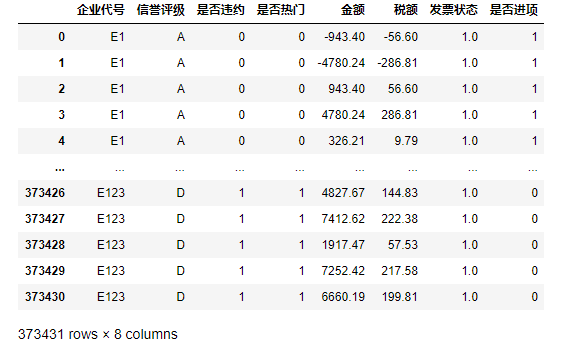
\includegraphics[width=0.7\textwidth]{Figure5-1}
        \caption{企业发票信息的特征矩阵}
        \label{fig51}
    \end{figure}
    \item 为了整理出神经网络训练需要的等大小特征矩阵并解决数据分布不均衡的问题,这一步我们采用了重采样的方法对每一个违约的企业生成了16000个特征矩阵,对每一个没有违约的企业生成了8000个特征矩阵,并贴上是否违约的对应标签。每个特征矩阵生成的策略是从企业的所有数据行中随机选择8行,并保留‘是否热门,金额 ,税额,发票状态,是否进项’共5列信息,组成一个$8 \times 5$的矩阵。这一步产生的结果示例如图\ref{fig52}。
    \begin{figure}[H]
        \centering
        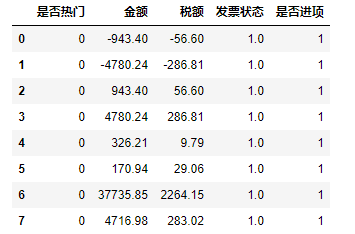
\includegraphics[width=0.7\textwidth]{Figure5-2}
        \caption{重采样后的特征矩阵}
        \label{fig52}
    \end{figure}
    \item 可以看到金额和税额这两列的值差异巨大,如果直接采用最简单的均值归一化方法,精度会超出计算机的表示范围,程序会无法识别,只好显示为NaN。这里采用的是正态归一化,采用$\mu$表示数据列的均值,用$\sigma$表示数据列的标准差,正态归一化的表达式为
    \begin{equation}
        x_i \gets \frac{x_i-\mu}{\sigma}
        \label{equa1}
    \end{equation}
    另外我们还对超出$\mu \pm 3\sigma$的数据进行了截断,使其分布情况更加合理。这一步得到的结果示例如图\ref{fig53}。
    \begin{figure}[H]
        \centering
        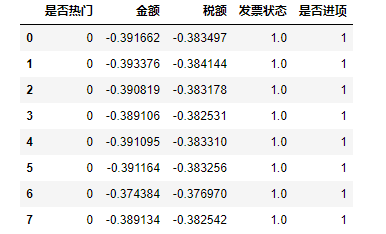
\includegraphics[width=0.7\textwidth]{Figure5-3}
        \caption{正态归一化后的特征矩阵}
        \label{fig53}
    \end{figure}
    \item 数据预处理部分共计整理出1200000个不同标签的特征矩阵,其中标签为1即有违约记录的企业有432000个特征图,数据量很大而且分布较为均匀,模型应该不会出现过拟合现象。
\end{itemize}

\subsection{问题一信贷风险量化分析}
由于信贷风险主要集中在中小微企业可能发生的违约上,所以对信贷风险的量化分析实际上可以转化为对企业违约率的分析上。首先根据前文数据预处理部分完成输入数据的整理,考虑到输入数据的可解释性差,所以我们选择了神经网络这种提取信息能力更强的模型。由于输入的矩阵为$8 \times 5$,所以使用简单的全连接网络足矣,没有必要使用卷积神经网络,网络结构如图\ref{fig54}。

\begin{figure}[H]
    \centering
    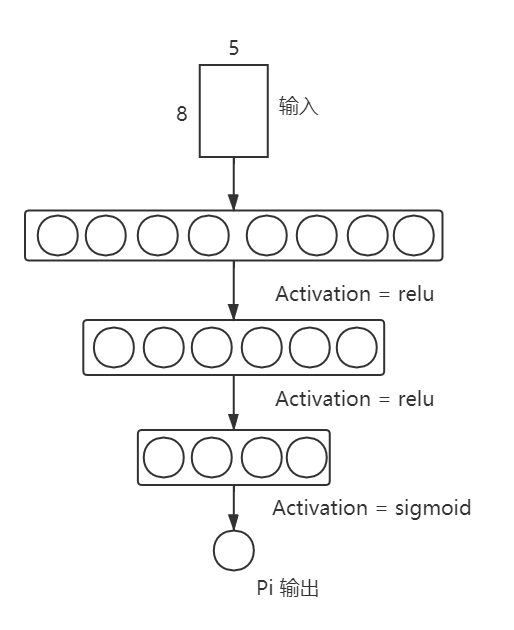
\includegraphics[width=0.7\textwidth]{Figure5-4}
    \caption{违约率预测的全连接神经网络}
    \label{fig54}
\end{figure}

网络一共四层,每层的神经元个数依次为8,6,4,1,第一层和第二层后面用relu函数\cite{ref3}(\ref{equarelu})进行激活,第三层后面接sigmoid激活函数(\ref{equasigm})输出一个0-1的概率值,将其与真实标签进行比较,算出误差并通过反向传播完成网络权重的更新,在训练200个epoch后模型正确率达到了64\%左右。
\begin{equation}
    \Phi(x) = max(0,x)
    \label{equarelu}
\end{equation}
\begin{equation}
    \Phi(x) = \frac{1}{1+e^{-x}}
    \label{equasigm}
\end{equation}

我们将从附件一中整理的1200000个特征矩阵喂入全连接神经网络预测得到输出概率,并对每一个企业的所有输出概率求均值,该值即为企业的预测违约率Pi,该值的大小可以衡量贷款风险的大小,每个企业的预测违约率Pi我们在附件一中具体给出。

\subsection{问题一信贷策略的制定}
我们还需要对这些企业制定在年度信贷总额固定时的信贷策略。根据上文问题一分析中的解释,我们将会给出每个企业的贷款额度、年利率作为该银行的信贷策略。
\subsubsection{信贷额度的确定}
首先是信贷额度Mi的确定,根据题目信息和生活经验,贷款风险低信誉评级高的企业应该分配更大的信贷额度,因此考虑使用上文预测的企业违约率对银行的信贷总额进行分配,其中信誉评级为D的企业不予分配贷款额度,满足违约率低的企业将会得到更多的贷款额度,具体的分配方式如式\ref{equalong1}。
\begin{equation}
\begin{split}
M_i=&
\begin{cases}
\frac{1-P_i}{P_{sum}}\times K, & Q_i \ne 'D'\\
0 & Q_i = 'D' \\
\end{cases} \\
\mbox{其中} &  P_{sum} = \sum_{j=1}^{123} a_j (1-P_j) \\
 a_j =& 
\begin{cases}
1 & Q_j \ne 'D' \\
0 & Q_j = 'D'\\
\end{cases}
\end{split}
\label{equalong1}
\end{equation}
我们首先求出某个信誉评级不为D的企业的信誉率占所有信誉评级不为D的企业的信誉率之和的比例,其中信誉率为$1-P_i$,然后根据这一比例划分银行的信贷总额,注意对不满足贷款额度为10\textasciitilde 100万元的值进行截断,最终可以得到每个企业的贷款额度$M_i$。
\subsubsection{年利率的确定}
在信贷额度确定的情况下,年利率的确定$\rho_i$可以看作一个最优化问题,优化目标是企业的年收益最大和客户流失率最小。根据题目信息和生活经验,贷款风险低信誉评级高的企业应该给予一定的年利率优惠。综合分析后,我们的策略是先根据最优化目标求得特定信誉评级下的基准年利率,然后按照企业的预测违约率进行微调,当然信誉评级为D的企业没必要考虑年利率的取值,并且我们仅考虑影响年收益和客户流失率的众多影响因素中的年利率设置因素。


首先求特定信誉评级下的基准年利率。优化目标是银行的年收益最大和客户流失率最小。银行在借贷过程中的主要收益是来自于借贷后产生的利息,但是每笔钱还需要扣除银行的平均运营成本。客户的流失率我们在假设中写到其仅仅与年利率的确定有关,所以相关的值直接查附件三即可得到。我们的优化目标可以表示为
\begin{equation}
    \begin{split}
    & \max \sigma(M_i \rho_i) - \sigma(F_j(\rho_i))
    \\
    \mbox{其中} &  \sigma(x_j) = \frac{\sum_{i=1}^{j}x_i}{\sum_{i=1}^{n}x_i} \\
    \end{split}
    \label{equalong2}
\end{equation}
式子中,$\rho_i$ 为年利率,$M_i$为企业i的信贷额度,$N$为银行每年平摊在每笔贷款上的固定成本,
$F_j(\rho_i)$表示年利率为$\rho_i$信誉评级为j时的客户损失率,$\sigma$表示归一化函数,其目的是为了消除银行年收益和客户流失率之间的量纲差异影响。前面一项表示的是归一化后的银行年收益,目标是使其最大,后面一项是归一化后的客户流失率,目标是使其最小,中间用减号连接,目标转化为合式最大。

接下来我们开始求解上述优化问题,根据附件3中可以发现,随着年利率的增大客户流失率逐渐增大,同等年利率下信誉评级为A的企业客户流失率始终最大。接着通过细致地考虑发现,由于归一化函数的作用,容易推导出最优化目标可以忽视$M_i$和N影响。因此我们只需要首先按照上面的归一化函数将年利率,信誉评级为A,B,C的客户损失率映射到同一个量纲的空间,然后在这个找到能够使得年利率和信誉评级为A,B,C的客户损失率的差值最大的年利率,求得的这三个年利率分别为信誉评级为A,B,C的基准年利率
$\beta_A$=0.0585,$\beta_B$=0.0625,$\beta_C$=0.0665,可以观察到满足信誉等级越高,基准年利率越低。

然后按照企业的预测违约率进行微调,微调的原则是信誉等级为C的不调整,信誉等级为A,B的企业按照式\ref{lilv}微调:
\begin{equation}
    \rho_i \gets \rho_i - (1 - P_i) \cdot \rho_\triangle
    \label{lilv}
\end{equation}

其中$P_i$为预测的违约率,$\rho_\triangle$为查阅资料设定的先验值,参考值为0.01,另外要注意如果年利率不满足4\% \textasciitilde 15\%则需要进行截断。第二问我们会具体使用这个模型,并将每个企业的信贷额度和年利率保存在附件二中。

\subsection{问题二模型建立与求解}
问题二相较于问题一的差别主要是给出的302家企业没有贷款记录据预处理方式得到模型的输入特征矩阵和对应的标签,喂入全连接网络模型后得到每一个企业的预测违约率。与问题一不同的是,这302家企业的信誉评级数据缺失。
,并且信贷总额被设置为1亿元,基本思路和问题一保持一致 。
我们这里介绍一下这302家企业的信誉评级的补全策略。首先提取出附件一中企业的信誉等级与违约率的关系,然后对提取出的表按照违约率排序,然后通过人工观察的方式确定三个合适违约率作为分位点,通过分位点划分即可确定企业的信誉评级,满足违约率越小的企业信誉等级越高,具体内容如式\ref{pingji123}。



\begin{equation}
    Q_i = 
    \begin{cases}
        'A' & P_i < 0.9716 \\
        'B' & 0.9716 \leq P_i < 0.9929 \\
        'C' & 0.9929 \leq P_i < 0.9967 \\
        'D' & P_i \geq 0.9967
    \end{cases}
    \label{pingji123}
\end{equation}

通过分析附件一中的原始数据,我们发现大部分信誉评级为D的企业都有违约记录,所以我们可以先根据附件一测试模型准确度。结果发现,我们预测的有违约的企业即信誉评级为D的企业共有22家,其中有14家企业确实发生了违约记录。

按照上述信誉评级的补全策略我们对附件二中的302家企业的信誉评级以及预测是否违约进行了补全,并保存在了附件二中,我们共评级了63家D企业,79家C企业,93家B企业,67家A企业,这里展示部分结果如图\ref{figpingji}:


\begin{figure}[H]
    \centering
    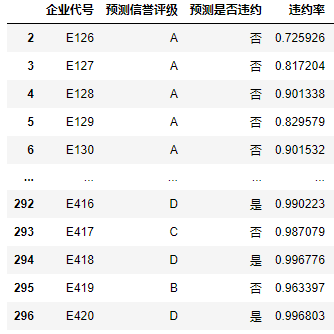
\includegraphics[width=0.7\textwidth]{fig579}
    \caption{企业违约率以及信誉评级估计}
    \label{figpingji}
\end{figure}

对这302家企业的信誉评级进行补全后,最后按照与问题一相同的方法确定每一个企业的贷款策略,我们将求得的每个企业的信贷额度和年利率保存在了附件二中,
这里展示部分结果表\ref{table23445}:

\begin{table}[H]
    \begin{center}
    \begin{tabular}{|c|c|c|}
        \hline
    企业代号 & 信贷额度 & 年利率\\
    \hline
    $E124$ & 1000000    & 0.04979357\\
    $E125$ & 1000000 & 0.0485\\
    $E126$ & 1000000 & 0.055759258\\
    $E127$ & 1000000 & 0.056672045    \\
    $E128$ & 567867.1643 & 0.057513380\\
    \vdots & \vdots & \vdots\\
    $E421$ & 0 & 0\\
    $E422$ & 0 & 0\\
    $E423$ & 0 & 0\\
    $E424$ & 0 & 0\\
    $E425$ & 0 & 0\\
    \hline
    \end{tabular}
    \end{center}
    \caption{附件2企业信贷额度以及年利率}
    \label{table23445}
    \end{table}

    最后我们对每个企业的信贷额度和年利率画出了散点图\ref{sandian1}与图\ref{sandian2}。
    \begin{figure}[H]
        \centering
        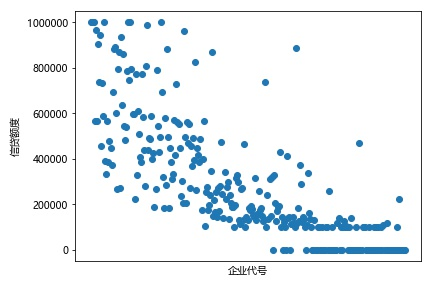
\includegraphics[width=0.7\textwidth]{sandian1}
        \caption{附件2中302家企业信贷额度分布图}
        \label{sandian1}
    \end{figure}

    \begin{figure}[H]
        \centering
        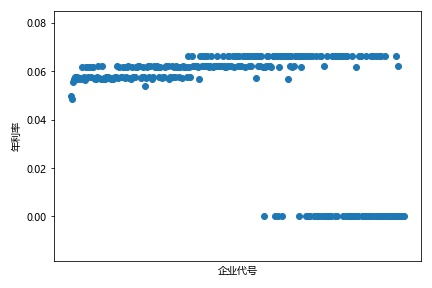
\includegraphics[width=0.7\textwidth]{sandian2}
        \caption{附件2中302家企业年利率分布图}
        \label{sandian2}
    \end{figure}
    可以发现信贷额度的分布较为均匀,年利率的分布关于信誉等级成阶梯分布。

%需要补充!
\subsection{问题三企业实力量化分析}
这里首先介绍我们的企业实力量化分析方案。我们考虑进项和销项发票信息中价税合计的统计量(最大值,均值,和)以及企业是否处于社会热门行业共7个因素,建立层次分析法模型得到302家企业的量化实力权重向量,向量值越大的企业代表相对实力越强。层次分析法(AHP)是对一些较为复杂、较为模糊的问题作出决策的简易方法,它特别适用于那些难于完全定量分析的问题。它是美国运筹学家T. L. Saaty 教授于上世纪70 年代初期提出的一种简便、灵活而又实用的多准则决策方法。具体的方案如下。



\subsubsection{层次定义及判断矩阵构造}
首先要把问题条理化、层次化,构造出一个有层次的结构模型,对于本题,我们选择了三层分析对象:

目标层O:选择综合实力最强的企业;

准则层C:选取了7项作为决定因素;

措施层P:附件二中302家企业。

其中决定因素的选取我们通过分析票据数据信息并查阅资料最终确定为:进项发票价税合计的最大值,进项发票价税合计的总值,进项发票价税合计的均值,销项发票价税合计的最大值,销项发票价税合计的总值,销项发票价税合计的均值,该行业是否为热门行业共7项,分别记为$\left[ in\_max,in\_sum,in\_avg,out\_max,out\_sum,out\_avg,ishot \right] $,后续描述我们会使用简称。
层次分析法的三层设置如图\ref{MultiLayer}。
\begin{figure}[H]
    \centering
    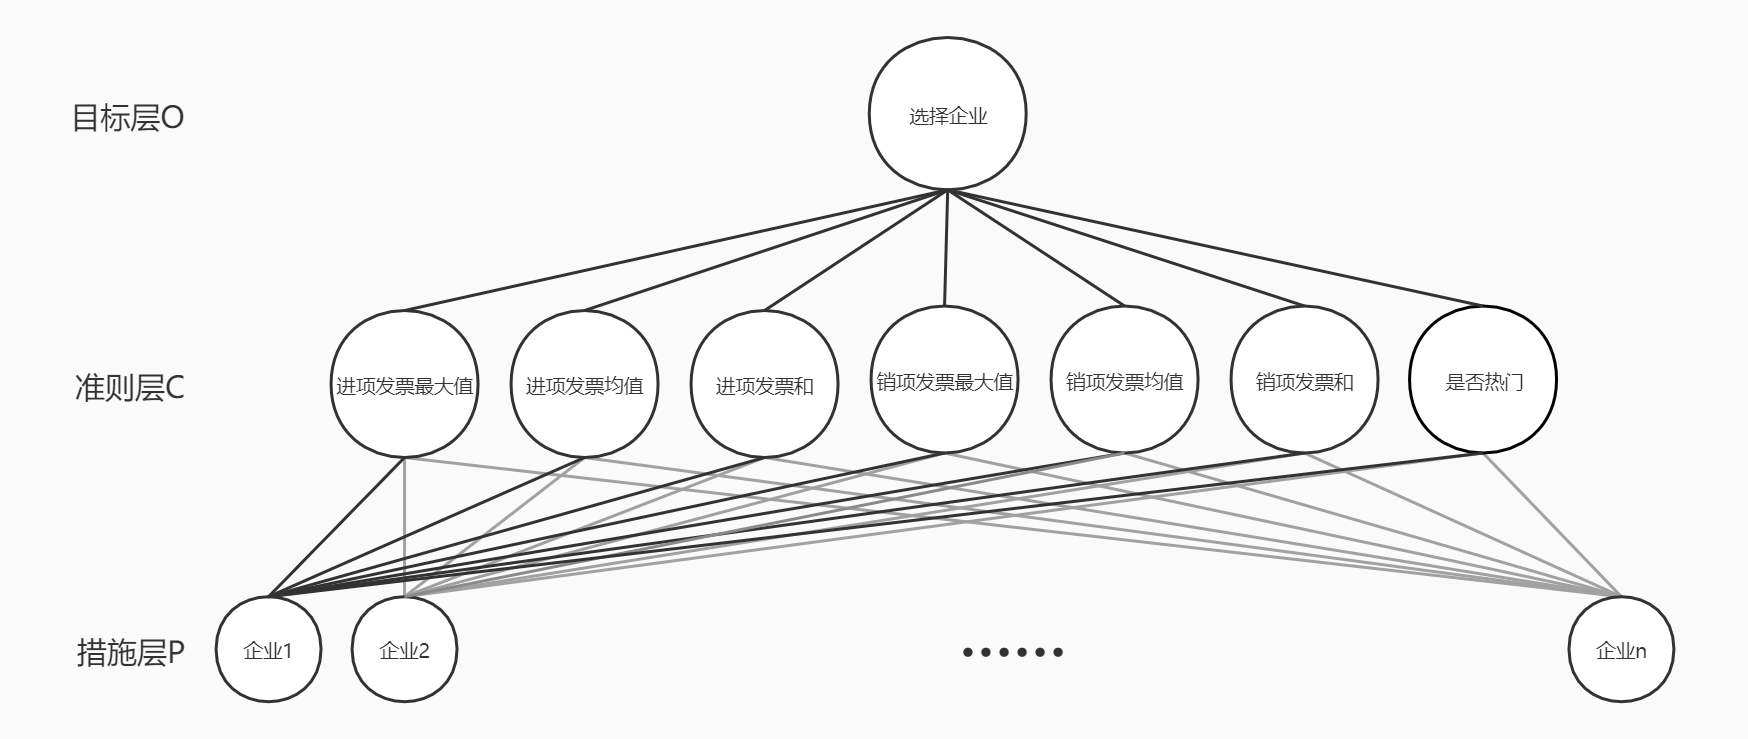
\includegraphics[width=0.7\textwidth]{MultiLayer}
    \caption{层次分析法的三层设置}
    \label{MultiLayer}
\end{figure}

然后构造因素的判断矩阵,层次结构反映了因素之间的关系,但准则层中的各准则在目标衡量中所占的比重并不一定相同,在决策者的心目中,它们各占有一定权重。在确定影响某因素的诸因子在该因素中所占的比重时,遇到的主要困难是这些比重常常不易定量化。 为此Saaty 等人建议可以采取对因子进行两两比较建立成对比较矩阵的办法。设现在要比较 n 个因子 $X = \left\{ x_1,\cdots, x_n \right\} $ 对某因素 $Z$ 的影响大小 ,即每次取两个因子 $x_i$ 和 $x_j$ ,以 $a_{ij}$ 表示 $x_i$ 和 $x_j$ 对因素$Z$的影响大小之比,全部比较结果用矩阵$A = (a_{ij} )_{n \times n} $表示,称 A 为 Z - X 之间的成对比较判断矩阵(简称判断矩阵)。容易看出,若 $x_i$ 与 $x_j$ 对 Z 的影响之比为 $a_{ij}$ ,则 $x_j$ 与 $x_i$ 对 $Z$ 的影响之比应为:
\begin{equation}
    a_{ji} = \frac{1}{a_{ij}}
\end{equation}

对于准则层的7x7判断矩阵,通过查阅金融领域相关资料,我们先对准则层的各准则重要程度进行了标度,重要程度的排序结果为:$$\left[ in\_max,in\_sum,in\_avg,out\_max,out\_sum,out\_avg,ishot\right]=[1,6,4,2,7,5,3]$$

数值越大代表对应因素的重要程度越高。对于比较矩阵A中的某一项$A\left[i\right]\left[j\right]:A\left[i\right]\left[j\right]=x_i/x_j$,其中$x_i$,$x_j$即为之前排序的重要程度。进而得到准则层的判断矩阵A,如表\ref{tablejudge}。

\begin{table}[H]
    \centering
    \begin{tabular}{|c|ccccccc|}%一个c表示有一列,格式为居中显示(center)
    \hline
        A & $B_1$ & $B_2$ & $B_3$ & $B_4$ & $B_5$ & $B_6$ & $B_7$   \\
    \hline 
    $B_1$  &  1   &$\frac{1}{6}$  &$\frac{1}{4}$  &$\frac{1}{2}$  &$\frac{1}{7}$  &$\frac{1}{5}$  &$\frac{1}{3}$\\
    $B_2$  &  6   &1              &$\frac{3}{2}$  &3              &$\frac{6}{7}$  &$\frac{6}{5}$  &2\\
    $B_3$  &  4   &$\frac{2}{3}$  &1              &2              &$\frac{4}{7}$  &$\frac{4}{5}$  &$\frac{4}{3}$\\
    $B_4$  &  2   &$\frac{1}{3}$  &$\frac{1}{2}$  &1              &$\frac{2}{7}$  &$\frac{2}{5}$  &$\frac{2}{3}$\\
    $B_5$  &  7   &$\frac{7}{6}$  &$\frac{7}{4}$  &$\frac{7}{2}$  &1              &$\frac{7}{5}$  &$\frac{7}{3}$\\
    $B_6$  &  5   &$\frac{5}{6}$  &$\frac{5}{4}$  &$\frac{5}{2}$  &$\frac{5}{7}$  &1              &$\frac{5}{3}$\\
    $B_7$  &  3   &$\frac{1}{2}$  &$\frac{3}{4}$  &$\frac{3}{2}$  &$\frac{3}{7}$  &$\frac{3}{5}$  &1\\
    \hline
\end{tabular}
    \caption{准则层的判断矩阵}
    \label{tablejudge}
\end{table}
对于措施层的7个$302 \times 302$判断矩阵,这里以第一个因素进项发票价税合计的最大值$in\_max$为例,其余的6个$302\times 302$判断矩阵可以通过分析另外6个因素求得。
首先是通过之前的数据预处理策略获得每一个企业的进项发票价税合计的最大值$in\_max$的取值,结果如下:

\begin{table}[H]
    
    \label{tablesymbol}
    \centering
    \begin{tabular}{|c|c|}   
    \hline
    企业代号 & 进项发票价税合计的最大值 \\
    \hline 
    $E124$  &  1109999.99\\
    $E125$  &  1109999.99\\
    $E126$  &  1082430.50\\
    $E127$  &  1029999.99\\
    $E128$  &  1000000.00\\
     \vdots &  \vdots \\  
    $E421$  &    10290.00\\
    $E422$  &     8350.00\\
    $E423$  &    33800.00\\
    $E424$  &     9765.00\\
    $E425$  &     9912.00\\
    \hline
    \end{tabular}
    \caption{附件2中302家企业的进项发票价税合计的最大值}
    \label{table2}
\end{table}

对于该$302 \times 302$的判断矩阵B某一项$B[i][j]: B[i][j] = \frac{in\_max[i]}{in\_max[j]}$,其中$in\_max[i]$,$in\_max[j]$分别表示企业代号i,j的$in\_max$取值。这里值得称赞的是,我们没有多此一举的去人工比较企业对因素的重要程度然后写出判断矩阵,而是直接复用了已有的数据取值,从而大大减少了工作量,直接计算即可求得措施层对$in\_max$因素的判断矩阵。

\subsubsection{层次单排序及一致性检验}
判断矩阵 A 对应于最大特征值$\lambda_{max}$的特征向量W ,经归一化后即为同一层次相应因素对于上一层次某因素相对重要性的排序权值,这一过程称为层次单排序。
上述构造成对比较判断矩阵的办法虽能减少其它因素的干扰,较客观地反映出一对因子影响力的差别。但综合全部比较结果时,其中难免包含一定程度的非一致性。如果比较结果是前后完全一致的,则矩阵 A 的元素还应当满足:
\begin{equation}
    \begin{split}
        a_{ij}a_{jk} = a_{ik},  \quad  \forall i,j,k = 1,2,\cdots n \\
    \end{split}
\end{equation}
满足关系式的正互反矩阵称为一致矩阵。我们需要检验构造出来的(正互反)判断矩阵 A 是否严重地非一致,以便确定是否接受 A 。 

这里给出定理:n 阶正互反矩阵 A 为一致矩阵当且仅当其最大特征根$\lambda_{max} = n$ ,且当正互反矩阵 A 非一致时,必有 $\lambda_{max}> n$ 。 根据该定理,我们可以由$\lambda_{max}$ 是否等于 n 来检验判断矩阵 A 是否为一致矩阵。由于特征根连续地依赖于$a_{ij}$ ,故 $\lambda_{max}$ 比 n 大得越多, A 的非一致性程度也就越严重。
据此提出判断矩阵的一次一致性检验步骤如下:
\begin{itemize}
    \item 计算一致性指标$CI = \frac{\lambda_{max}-n}{n-1}$。
    \item 查找相应的平均随机一致性指标RI。对 $n = 1,,9$,Saaty给出了RI的值,如表\ref{RIde}。
    \begin{table}[H]
        \label{tablesymbol}
        \centering
        \begin{tabular}{c|ccccccccc}   
        \hline 
        $n$  &  1 & 2 & 3 & 4 & 5 & 6 & 7 & 8 & 9\\
        \hline
        $RI$  &  0 & 0 & 0.58 & 0.90 & 1.12 & 1.24 & 1.32 & 1.41 & 1.45\\
        \hline
        \end{tabular}
        \caption{RI的值}
        \label{RIde}
    
    \end{table}
    RI 的值是这样得到的,用随机方法构造 500 个样本矩阵:随机地从$1,\cdots,9$ 及其倒
数中抽取数字构造正互反矩阵,求得最大特征根的平均值$\lambda^{'}_{max}$ ,并定义$RI = \frac{\lambda^{'}_{max}-n}{n-1}$。
    \item 计算一致性比例$CR = \frac{CI}{RI}$。
    当CR < 0.10 时,认为判断矩阵的一致性是可以接受的,否则应对判断矩阵作适当修正。
    \item 通过上续步骤对我们的一个准则层$7 \times 7$判断矩阵和措施层的7个$302 \times 302$判断矩阵进行一次一致性检验,结果都满足CR < 0.10,则这些正互反矩阵可以称为一致矩阵,我们可以接受这些判断矩阵的设定。 
\end{itemize}
\subsubsection{层次总排序及一致性检验}
上面我们得到的是一组元素对其上一层中某元素的权重向量。我们最终要得到各元素,特别是最低层中各方案对于目标的排序权重,从而进行方案选择。总排序权重要自上而下地将单准则下的权重进行合成。 
%层次总排序合成表
\begin{table}[H]
    \begin{center}
    \begin{tabular}{|c|c|c|c|c|c|}
    \hline
    \diagbox{层B}{层A} & $\mathop{}_{a_1}^{A_1}$  & $\mathop{}_{a_2}^{A_2}$ & $\mathop{}_{...}^{...}$ & $\mathop{}_{a_m}^{A_m}$ & B层总排序权值 \\
    \hline
    $B_1$ & $b_{11}$ & $b_{12}$ & ... & $b_{1m}$ & $\sum_{j=1}^mb_{1j}a_j$ \\
    $B_2$ & $b_{21}$ & $b_{22}$ & ... & $b_{2m}$ & $\sum_{j=1}^mb_{2j}a_j$ \\
    ... & ... & ... & ... & ... & ... \\
    $B_n$ & $b_{n1}$ & $b_{n2}$ & ... & $b_{nm}$ & $\sum_{j=1}^mb_{nj}a_j$ \\
    \hline
    \end{tabular}
    \caption{层次总排序合成表}
    \label{hechengbiao}
    \end{center}
\end{table}
设上一层次( A 层)包含$A_1,\cdots,A_m$ 共 m 个因素,它们的层次总排序权重分别为$a_1,\cdots,a_m$。又设其后的下一层次( B 层)包含 n 个因素 $B_1,\cdots, B_n$ ,它们关于 $A_j$ 的层次单排序权重分别为$b_{1j} ,\cdots,b_{nj}$ (当 $B_i$ 与 $A_j$ 无关联时,$ b_{ij} = 0$ )。现求 B 层中各因素关于总目标的权重,即求 B 层各因素的层次总排序权重$b_1,\cdots,b_n$ ,计算按上表所示方式进行,如式\ref{equabi}:
\begin{equation}
    b_i = \sum_{j = 1}^{m}b_{ij}a{j}, \quad i = 1,\cdots,n
    \label{equabi}
\end{equation}

通过准则层$7 \times 7$判断矩阵,我们可以得出准则层各准则的权重向量,如式\ref{equation7x7}:
\begin{equation}
    \begin{split}
    & \left[in\_max in\_sum in\_avg out\_max out\_sum out\_avg ishot\right]= \\
    & \left[0.0357,0.2143,0.1429,0.0714,0.2500,0.1786,0.1071\right]
    \end{split}
    \label{equation7x7}
\end{equation}

通过措施层的302x302判断矩阵分别求得所有企业对每个因素的权重向量,进而按照表\ref{hechengbiao},
所示方式求得302家企业对上一层7个因素的总目标的权重,该权重的值即可视为企业的实力$\theta_i$,权重值越大代表企业实力越强。

对层次总排序也需作一致性检验,检验仍象层次总排序那样由高层到低层逐层进行。这是因为虽然各层次均已经过层次单排序的一致性检验,各成对比较判断矩阵都已具有较为满意的一致性。但当综合考察时,各层次的非一致性仍有可能积累起来,引起最终分析结果较严重的非一致性。

设 B 层中与Aj 相关的因素的成对比较判断矩阵在单排序中经一致性检验,求得
单排序一致性指标为$CI\left(j\right)$ ,$\left(j = 1,...,m\right)$,相应的平均随机一致性指标为 $RI\left(j\right)$($CI\left(j\right)$、$RI\left(j\right)$ 已在层次单排序时求得),则 B 层总排序随机一致性比例为:


\begin{equation}
    CR = \frac{\sum^{m}_{j=1}CI\left(j\right)a_j}{\sum^{m}_{j=1}RI\left(j\right)a_j}
\end{equation}

当CR < 0.10 时,认为层次总排序结果具有较满意的一致性并接受该分析结果。 

所有企业的实力权重保存在了附件中,以下为部分取值示例:

\begin{table}[H]
    \begin{center}
    \begin{tabular}{|c|c|c|}
        \hline
    企业代号 & 企业名称 & 实力权重\\
    \hline
    $E124$ & 个体经营E124 & 0.048507\\
    $E125$ & 个体经营E125 & 0.055684\\
    $E126$ & 个体经营E126 & 0.01541\\
    $E127$ & 个体经营E127 & 0.010346\\
    $E128$ & 个体经营E128 & 0.005679\\
    \vdots & \vdots & \vdots\\
    $E421$ & ***保温材料有限公司 & 0.000256\\
    $E422$ & ***童装店          & 0.000205\\
    $E423$ & ***通风设备有限公司 & 0.000682\\
    $E424$ & ***贸易有限公司 & 0.0007\\
    $E425$ & ***商贸有限公司 & 0.000654\\
    \hline
    \end{tabular}
    \end{center}
    \caption{附件2企业实力权重}
    \label{tablecenci}
    \end{table}

\subsection{问题三突发因素下信贷策略调整}
通对突发因素下的信贷策略进行调整,使模型更加接近于真实情况,实际上只需对之前模型的预测违约率进行人工微调即可。我们可以首先根据突发因素的影响行业确定违约率的修正方向,不同类型的企业修正方向是不同的;然后根据企业实力和突发因素的剧烈程度确定违约率的修正范围。根据以上分析,我们对之前的模型加以调整,对违约率$P_i$加一个偏置项,调整违约率的公式如下:

\begin{equation}
    \begin{split}
         P_i &\gets  P_i + b_i \left(1-\theta_i \right) \alpha \\
        \mbox{其中} b_i & = 
        \begin{cases}
            -1 & \mbox{突发因素促进企业发展} \\
            0 & \mbox{突发因素对企业无影响} \\
            1 &\mbox{ 突发因素抑制企业发展} \\
        \end{cases}
    \end{split}
\end{equation}

其中$b_i$代表了预测违约率的调整方向,$\theta_i$为层次分析法求得的企业i的实力权重,$\alpha$ 突发因素对违约率的基准影响程度,这个值需要根据发生的具体突发因素来确定。公式满足常识,综合实力强的企业受突发因素的影响较小,综合实力弱的企业受突发因素的影响较大,另外如果突发因素客观上非常剧烈,对社会影响很大,那么对应的违约率的修正范围也会更大。

最后使用微调过的预测违约率按照与问题二相同的方法确定最终的信贷策略,这里我们假设突发因素为新冠病毒疫情,取$\alpha = 0.01$,疫情的爆发等对医疗有关企业有促进作用,而对食品有关企业有抑制作用,据此求得每个企业经过修正的违约率进而求得银行的信贷策略,所有结果保存在了附件三中,以下部分结果示例:

\begin{figure}[H]
    \centering
    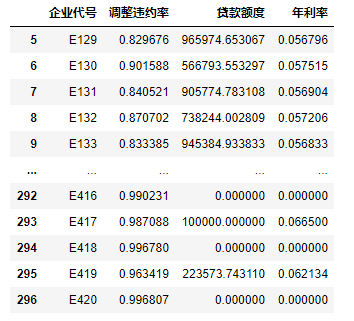
\includegraphics[width=0.7\textwidth]{figjieguo}
    \caption{302家企业突发因素下的信贷调整结果}
    \label{figjieguo}
\end{figure}

\section{模型评价和推广}
\subsection{模型优点}
\begin{itemize}
    \item 从企业真实票据数据出发进行建模分析,解决了信息受限情况下的银行信贷策略的制定,使对申请贷款的企业的综合实力有较为清晰的认识,减少了借贷双方的不透明度。
    \item 数据预处理部分创新性地采用重采样的方法解决类别分布不均衡的问题,采用正态归一化的方法处理计算机无法处理的越界数据,最终提取出了1200000个带有是否违约的标签的$8 \times 5$的特征矩阵,数据量足够神经网络训练。
    \item 运用全连接的神经网络构造二分类模型对企业的违约率进行预测。由于普通的线性模型或者树模型模型自身的拟合能力较弱,可能无法从肉眼上毫无规律可循的票据数据中提取出有用信息。由于输入的特征矩阵维度比较低,只有$8 \times 5$大小,所以没有必要用到卷积神经网络,使用全连接神经网络即可。
    \item 运用层级分析法建立企业实力分析的量化模型,将复杂,模糊的问题量化讨论,提出了一种简便、灵活而又实用的多准则决策方法。
\end{itemize}
\subsection{模型改进}
\begin{itemize}
    \item 我们假设银行给予中小微企业的信贷额度都能被企业完全使用,以便我们计算信贷策略确定时的银行年收益,但是实际中少部分情况并非如此,也即企业只使用了银行分配的部分贷款额度。我们可以采取的改进策略是提高分配的银行贷款总额,比如分配110\%的实际银行贷款总额,当然具体的超实际分配总额需要根据经验确定,太大可能导致资金熔断,太小可能导致资金闲置。我们的期望目标是,即使有部分企业只使用了银行分配的部分贷款额度,银行也能尽可能的使用完实际贷款总额,最大化年收益。
    \item 全连接网络精度不高,在训练200个epoch后模型正确率达到了64\%左右,这个显然没有达到预期,我们初步分析后认为大概与输入数据的自身的可解释性很差有关,解决的方案是通过查阅资料搜寻每一个企业的更多信息进行外部数据扩充,从而增大输入特征矩阵的维度,以便神经网络能选择更多有效的信息来预测企业的违约率。另外,还有可能是网络本身的结构比较简单造成的正确率低问题,可以采取的策略包括增加网络宽度和深度,在每层的后面添加正则化层,使用DROPOUT技术减少过拟合等等,这些技术有机会可以尝试一下对违约预测正确率的影响。
    \item 虽然我们的措施层$302 \times 302$矩阵是从数据中推导出来的,但是准则层的7x7矩阵却只能人为确定,评价标准是个人心目中的重要程度,这样难免造成与真实情况一定的偏差。因此,构造判断矩阵应由经验丰富、判断力强的专家给出,需要我们查阅更多资料。
\end{itemize}
    %\item 我们假设银行给予中小微企业的信贷额度都能被企业完全使用,以便我们计算信贷策略确定时的银行年收益,但是实际中少部分情况并非如此,也即企业只使用了银行分配的部分贷款额度。我们可以采取的改进策略是提高分配的银行贷款总额,比如分配110\%的实际银行贷款总额,当然具体的超实际分配总额需要根据经验确定,太大可能导致资金熔断,太小可能导致资金闲置。我们的期望目标是,即使有部分企业只使用了银行分配的部分贷款额度,银行也能尽可能的使用完实际贷款总额,最大化年收益。
    %\item 全连接网络精度不高,在训练200个epoch后模型正确率达到了64\%左右,这个显然没有达到预期,我们初步分析后认为大概与输入数据的自身的可解释性很差有关,解决的方案是通过查阅资料搜寻每一个企业的更多信息进行外部数据扩充,从而增大输入特征矩阵的维度,以便神经网络能选择更多有效的信息来预测企业的违约率。另外,还有可能是网络本身的结构比较简单造成的正确率低问题,可以采取的策略包括增加网络宽度和深度,在每层的后面添加正则化层,使用DROPOUT技术减少过拟合等等,这些技术有机会可以尝试一下对违约预测正确率的影响。
    %\item 虽然我们的措施层$302 \times 302$矩阵是从数据中推导出来的,但是准则层的7x7矩阵却只能人为确定,评价标准是个人心目中的重要程度,这样难免造成与真实情况一定的偏差。因此,构造判断矩阵应由经验丰富、判断力强的专家给出,需要我们查阅更多资料。

\subsection{模型意义与推广}
本题中我们创新性的使用了神经网络处理是否违约这一二分类问题,对于银行来说,如果在放贷前就能预测出一个有参考价值的违约率,对于降低银行的运营费用,控制风险等方面将有着极高的经济价值。

我们通过包含重采样和正态归一化在内的数据预处理方法,提取出神经网络的输入特征矩阵,打破了文本表项数据一般使用线性模型或者树模型训练的常规思路,采用提取特征能力更强的神经网络建立模型,这一部分方案可以推广到更多类似数据的处理方式上,为文本表格的数据提供了一种新的处理思路。

我们运用层次分析法建立企业实力分析的量化模型,将复杂,模糊的问题量化讨论,实际上不仅对于本题适用,对于类似的数据较为稀少的情况,我们可以采用层次分析法建立灵活而又实用的多准则决策方法。层次分析法常用于人才选拔和评价,生产决策,交通运输等问题的决策、评价、分析、预测中。

从社会意义上讲,信用的缺失导致的社会道德风气损坏以及成为制约中小企业业务健康发展的瓶颈之一。我们设计的这种“未卜先知”的预测方法,降低了信贷的信息成本和贷款费用,减少了商业银行和中小企业之间的信息不对称,对于形成全社会诚实守信的大环境有着积极的促进作用。



%参考文献
\begin{thebibliography}{9}%宽度9
    \bibitem{ref1}杨伟歧,商业银行中小企业信贷策略研究,山东大学硕士学位论文,2011-10
    \bibitem{ref2}Berger, A.N. and Udell, G.F., 1995.Relationship Lending and Lines of Credit in Small Firm Finance[j]. Journal of Business,(68):351-381
    \bibitem{ref3}Rectified Linear Units Improve Restricted Boltzmann Machines Vinod Nair.ResearchGate
    \bibitem{ref4}王文元,夏伯忠.新编会计大辞典:辽宁人民出版社,1991-01
\end{thebibliography}

\newpage
%附录
\begin{appendices}


\section{层次分析法--matlab 源程序}

\begin{lstlisting}[language=matlab]
    clc,clear
    fid=fopen('txt_total.txt','r');
    n1=7;n2=123;
    a=[];
    for i=1:n1
    tmp=str2num(fgetl(fid));
    a=[a;tmp]; %读准则层判断矩阵
    end
    for i=1:n1
    str1=char(['b',int2str(i),'=[];']);
    str2=char(['b',int2str(i),'=[b',int2str(i),';tmp];']);
    eval(str1);
    for j=1:n2
    tmp=str2num(fgetl(fid));
    eval(str2); %读方案层的判断矩阵
    end
    end
    ri=[0,0,0.58,0.90,1.12,1.24,1.32,1.41,1.45]; %一致性指标
    [x,y]=eig(a);
    lamda=max(diag(y));
    num=find(diag(y)==lamda);
    w0=x(:,num)/sum(x(:,num));
    cr0=(lamda-n1)/(n1-1)/ri(n1)
    for i=1:n1
    [x,y]=eig(eval(char(['b',int2str(i)])));
    lamda=max(diag(y));
    num=find(diag(y)==lamda);
    w1(:,i)=x(:,num)/sum(x(:,num));
    %cr1(i)=(lamda-n2)/(n2-1)/ri(n2);
    end
    ts=w1*w0
    %cr=cr1*w0
 \end{lstlisting}
 \section{支撑文件列表}
 \begin{itemize}
     \item 附件一:123家企业的信誉评级,是否违约,预测信誉评级,预测是否违约,违约率,实力权重的信息。
     \item 附件二:302家企业的预测信誉评级,预测是否违约,违约率,实力权重,贷款额度,年利率的信息。
     \item 附件三:302家企业突发因素下的预测信誉评级,预测是否违约,调整违约率,实力权重,调整贷款额度,调整年利率的信息。
 \end{itemize}
\end{appendices}

\end{document} 